\documentclass[12pt, 
%twoside
]{article}
\usepackage{braket}
\usepackage{ctex}%add Chinese supports
\usepackage{upgreek}%add special greek symbols
\usepackage{graphicx}%include figure files
\usepackage{tikz}
\usepackage{wrapfig}
%\usepackage{subfigure}
\usepackage{amsmath}%add special math symbols
\usepackage{amssymb}
\usepackage{bm}%bold math
%\usepackage{xfrac}%add special fraction supports
\usepackage{color}
\usepackage{makecell}
\usepackage{multirow}
\newcommand{\tabincell}[2]{\begin{tabular}{@{}#1@{}}#2\end{tabular}} 
\usepackage[colorlinks, 
linkcolor=black,
anchorcolor=blue, citecolor=blue, urlcolor=blue]{hyperref}% add hypertext capabilities
\usepackage{geometry}
\geometry{a4paper, centering, scale=0.8}

\usepackage{fancyhdr}
\pagestyle{fancy}
%\fancyhead[CE]{}
%\fancyhead[CO]{}
%\fancyhead[RO]{\thepage} 
%\fancyhead[LE]{\thepage} 
%\fancyhead[LO]{\leftmark}
%\fancyhead[RE]{\leftmark}

\lhead{}
\chead{}
\rhead{\leftmark}
\renewcommand{\headrulewidth}{0.4pt}
\setlength{\headheight}{15pt}
\newcommand{\dbar}{\mathrm{d}\hspace*{-0.2em}\bar{}\hspace*{0.1em}}
%
%  Created by WW on 11/27/19
%  Copyright © WW. All rights reserved.
%

\begin{document}\fangsong
	\title{{\bf Notes for GRE Physics}}
	\author{~\\汪巍\footnote{Copyright \copyright ~Wei Wang 2019. All rights reserved.}}
	\date{2019-11}
	\maketitle

	\thispagestyle{empty}

	
	\newpage
	\fancyfoot{\empty}
	\begin{center}
	{\large\bf Preface}
	\end{center}

		%\addcontentsline{toc}{section}{Preface}%add Abstract into Contents.
		For test takers of GRE Physics, there are few materials to prepare. I took the test on Oct. 26, 2019 in Shanghai and got a full mark 990 (95\%). Therefore, I plan to organize my notes based on Jeff's version...
		~\\

		
	\begin{figure}[h]
	\vspace{2cm}
	\flushright
	
\includegraphics[width=.15\textwidth]{sign.png}
	\end{figure}
	\vspace{-0.5cm}
	\hfill Wei Wang

	\hfill Nov. 2019 at Tongji University

	{
	\lhead{}
	\chead{}
	\rhead{Preface}
	}
	
	\newpage
	\tableofcontents
	\thispagestyle{empty}% This page is not counted in the page number

	\newpage
	\fancyfoot[C]{\thepage}
	\setcounter{page}{1}%start page number counter...

	

	\lhead{}
	\chead{}
	\rhead{\leftmark}

\section{Classic Mechanics}
\addcontentsline{toc}{subsection}{1.1 General Knowledge}%add to contents
\noindent1. 保守力:
$
	\nabla\times\vec{F}=0\Rightarrow\vec{F}=-\nabla U.
$

\noindent2. 抛体:Projectile.~\\

\noindent3. 弹簧串联:$\dfrac{1}{k_t}=\dfrac{1}{k_1}+\dfrac{1}{k_2}$; 并联:$k_t=k_1+k_2$;
\begin{equation*}
	\lambda=\frac{R}{2}\sqrt{\frac{C}{L}}~~~\left\{
		\begin{array}{l}
			>1:\text{overdamped  过阻尼;}\\
			=1:\text{critically damped 临界阻尼;}\\
			<1:\text{underdamped 欠阻尼}\Rightarrow\text{频率:}~\omega_d=\omega_0\sqrt{1-\dfrac{b}{4mk}}:b\text{阻尼系数.}\\
		\end{array}
		\right.
\end{equation*}

\noindent4. 冲量:impulse.~\\

\noindent5. 转动惯量:the moment of inertia; 支点:fulcrum; 单摆:pendulum$\Rightarrow\omega=\sqrt{\dfrac{g}{l}}$.~\\

\noindent6. centripetal: 向心的;\\
			\phantom{~~~~}centrifugal: 离心.\\

\noindent7. 科里奥利力:$\vec{F}_c=-2m\vec{\omega}\times\vec{v}$~\\

\noindent8. 天体:$E=\dfrac{1}{2}mv^2+V(r)=\dfrac{1}{2}m\dot{r}^2+\dfrac{1}{2}mr^2\dot{\theta}^2+V(r)$,而$L=mr^2\dot{\theta}$,

~~~~故$E=\dfrac{1}{2}m\dot{r}^2+\dfrac{L^2}{2mr^2}+V(r)=\dfrac{1}{2}m\dot{r}^2+V_{eff}$
~\\

\noindent9. 伯努利方程:$\dfrac{1}{2}\rho v^2+\rho gh+P=C$;
~\\\phantom{~~~~}不可压缩流体:$v_iA_i=C$;
~\\\phantom{~~~~}斯托克斯定律(球体):$F_{drag}=-6\pi\mu Rv_s$, $\mu$为黏度系数,$v_s$为下落最终速度.\\
\begin{wrapfigure}{r}{.4\textwidth}
\hspace{0.8cm}
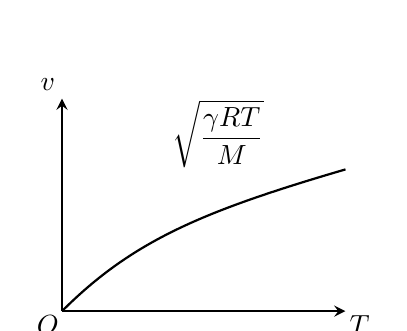
\begin{tikzpicture}[scale=0.9]
	\coordinate (O) at (0,0);
	\coordinate (A) at (0,3);
	\coordinate (B) at (4,0);
	\draw[thick, -stealth] (O)--(B);
	\draw[thick, -stealth] (O)--(A);
	\node at (-0.2,-0.2) {$O$};
	\node at (4.2,-0.2) {$T$};
	\node at (-0.2,3.2) {$v$};
	\draw[thick] (0,0) .. controls (1,1) and (2,1.414) .. (4,2);
	\node at (2.2,2.5) {$\sqrt{\dfrac{\gamma RT}{M}}$};
\end{tikzpicture}
	\caption{理想气体中声波传播速度.}
\label{fg:1}
\end{wrapfigure}
\noindent10. 波在弦中传播速度:$v=\sqrt{\dfrac{T}{\mu}}$, $T$为弦中张力, \phantom{~~~~~~}$\mu$为弦线密度;
~\\
\addcontentsline{toc}{subsection}{1.2 Mechnical Wave}%add to contents

\noindent11. 球面波强度:$I=\dfrac{P_s}{4\pi r^2}\propto\dfrac{1}{r^2}$; ~\\\phantom{~~~~~}声强级:$\beta=10\log\dfrac{I}{I_0}$(dB), $I_0$为$10^{-12}$;~\\
\phantom{~~~~~}理想气体中声波传播速度:$v=\sqrt{\dfrac{\gamma RT}{M}}\propto\sqrt{T}$, \\\phantom{~~~~~}如图\ref{fg:1}所示.

\noindent12. 允许的频率数=系统的自由度~\\
\begin{wrapfigure}{r}{.4\textwidth}
\vspace{-1cm}
\hspace{0.8cm}
\begin{tikzpicture}[scale=0.9]
	\draw[domain=0:3.141] plot(\x,{0.3*cos(\x r)});
	\draw[domain=0:3.141] plot(\x,{-0.3*cos(\x r)});
	\draw[domain=0:3.141] plot(\x,{0.3*sin(1.5*\x r)-1});
	\draw[domain=0:3.141] plot(\x,{-0.3*sin(1.5*\x r)-1});
	\draw[thick] (0,-0.6)--(0,-1.4);
	\draw (0,-0.65)--(-0.1,-0.75);
	\draw (0,-0.75)--(-0.1,-0.85);
	\draw (0,-0.85)--(-0.1,-0.95);
	\draw (0,-0.95)--(-0.1,-1.05);
	\draw (0,-1.05)--(-0.1,-1.15);
	\draw (0,-1.15)--(-0.1,-1.25);
	\draw (0,-1.25)--(-0.1,-1.35);
	\node at (4.5,0) {两端开口};
	\node at (4.5,-1) {一端开口};
	\end{tikzpicture}
\end{wrapfigure}

\noindent13. 两端开口管:$L=n\dfrac{\lambda}{2}$;
\\\phantom{~~~~}一端开口管:$L=\dfrac{2n+1}{4}\lambda$
\\\phantom{~~~~}harmonics: $n=Round\left(\dfrac{f_2}{f_1}\right)$;beats$=n\times f_1-f_2$.
~\\

\noindent14. 火箭运动:$m\dfrac{\mathrm{d}v}{\mathrm{d}t}+u\dfrac{\mathrm{d}m}{\mathrm{d}t}=0$, $u$为相对速度。~\\

\addcontentsline{toc}{subsection}{1.3 Analytical Mechanics}%add to contents
\noindent15. 分析力学:
~\\\phantom{~~~~}拉格朗日函数:$L(q,\dot{q},t)=T-U$.
~\\\phantom{~~~~}action作用函数:$S=\displaystyle\int L\mathrm{d}t$.
~\\\phantom{~~~~}哈密顿原理:actual path满足$\delta\displaystyle\int L\mathrm{d}t=0$, 即actual作用函数$S$是极值。
~\\\phantom{~~~~}拉格朗日方程:
\[
	\frac{\mathrm{d}}{\mathrm{d}t}\left(\frac{\partial L}{\partial\dot{q}}\right)-\frac{\partial L}{\partial q}=0,~\text{广义动量:}~p=\frac{\partial L}{\partial\dot{q}},
\]
\phantom{~~~~}类似于牛顿第二定律:$ma=\dfrac{\mathrm{d}p}{\mathrm{d}t}=F$.
~\\\phantom{~~~~}哈密顿量:$H(q,p,t)=\displaystyle\sum_i p_i\dot{q_i}-L$.
~\\\phantom{~~~~}正则方程:
\[
	\dot{q}=\frac{\partial H}{\partial p},~\dot{p}=-\frac{\partial H}{\partial q},~\frac{\partial H}{\partial t}=-\frac{\partial L}{\partial t},
\]
\phantom{~~~~}其中第二个式子应用了拉格朗日方程和广义动量的定义:
$$\frac{\partial H}{\partial q}=-\frac{\partial L}{\partial q}=-\frac{\mathrm{d}}{\mathrm{d}t}\left(\frac{\partial L}{\partial\dot{q}}\right)=-\dot{p}.$$

\newpage
\section{Electrodynamics}
\noindent1. 毕奥·萨伐尔定律:$\displaystyle B=\frac{\mu_0}{4\pi}\int\frac{I\times\hat{r}}{r^2}\mathrm{d}l=\frac{\mu_0}{4\pi}\int\frac{J\times\hat{r}}{r^2}\mathrm{d}V$.
~\\

\addcontentsline{toc}{subsection}{2.1 Maxwell Equations}%add to contents
\noindent2. Maxwell方程组:
\[
	\left\{
	\begin{array}{l}
		\displaystyle\nabla\times\vec{E}=-\frac{\partial\vec{B}}{\partial t}; \\
		\nabla\cdot\vec{E}=\dfrac{\rho}{\varepsilon_0};\\
		\nabla\cdot\vec{B}=0;\\
		\nabla\times\vec{B}=\mu_0\vec{J}+\mu_0\varepsilon_0\dfrac{\partial\vec{E}}{\partial t}\Rightarrow~\text{位移电流:}~\vec{J}_D=\varepsilon_0\dfrac{\partial\vec{E}}{\partial t}=\dfrac{\partial\vec{D}}{\partial t}.
	\end{array}
	\right.
\]

\noindent3. 极化强度:$\vec{P}=\dfrac{\sum\vec{p_i}}{\Delta V}$,
~\\\phantom{~~~~}电位移矢量:
\[
	\left.
	\begin{array}{l}
		\vec{D}=\varepsilon_0\vec{E}+\vec{P}\\
		\vec{P}=\chi_e\varepsilon_0\vec{E}
	\end{array}
	\right\}\Rightarrow
\vec{D}=(1+\chi_e)\varepsilon_0\vec{E}=\varepsilon_r\varepsilon_0\vec{E}.
\]

\noindent4. 磁化强度:$\vec{M}=\dfrac{\sum \vec{m_i}}{\Delta V}$,
~\\\phantom{~~~~}磁场强度和磁感应强度的关系:$\vec{B}=\mu\vec{H}=(1+\chi_M)\mu_0\vec{H}=\mu_0\vec{H}+\mu_0\vec{M}$.
~\\

\noindent5. 在介质中:
~\\\phantom{~~~~~~}束缚电荷:$\rho_P=-\nabla\cdot\vec{P}\Rightarrow\sigma_P=-(P_2-P_1)$;
~\\\phantom{~~~~~~}净电荷:$\rho_P+\rho_f=\varepsilon_0\nabla\cdot\vec{E}\Rightarrow\sigma_P+\sigma_f=\varepsilon_0(E_2-E_1)$;
~\\\phantom{~~~~~~}自由电荷:$\rho_f=\nabla\cdot\vec{D}\Rightarrow\sigma_f=D_2-D_1$.
~\\

\noindent6. 在介质中:
\[
	\text{诱导电流}\left\{
	\begin{array}{l}
		\text{磁化电流:}\vec{J}_M=\nabla\times\vec{M};\\
		\text{极化电流:}\vec{J}_P=\dfrac{\partial\vec{P}}{\partial t},
	\end{array}
	\right.
\]
\phantom{~~~~}故:总电流=自由电流+诱导电流+位移电流,即$\dfrac{1}{\mu_0}\nabla\times\vec{B}=\vec{J}_f+\vec{J}_M+\vec{J}_P+\vec{J}_D$.
~\\

\noindent7. 介质中的Maxwell方程组:
\[
	\left\{
	\begin{array}{l}
		\nabla\times\vec{E}=-\dfrac{\partial\vec{B}}{\partial t};\\
		\nabla\cdot\vec{D}=\rho_f;\\
		\nabla\cdot\vec{B}=0;\\
		\nabla\times\vec{H}=\vec{J}_f+\dfrac{\partial\vec{D}}{\partial t}.
	\end{array}
	\right.
\]

\noindent8. 坡印廷矢量:$\vec{S}=\vec{E}\times\vec{H}$.
~\\\phantom{~~~~}欧姆定律微观形式:$\vec{J}=\sigma\vec{E}$.
~\\

\noindent9. 电磁场的变值关系:
\[
	\left\{
	\begin{array}{l}
		\vec{e}_n\times(\vec{E}_2-\vec{E}_1)=0;\\
		\vec{e}_n\times(\vec{H}_2-\vec{H}_1)=\vec{\alpha};\\
		\vec{e}_n\cdot(\vec{D}_2-\vec{D_1})=\sigma_f;\\
		\vec{e}_n\cdot(\vec{B}_2-\vec{B}_1)=0.
	\end{array}
	\right.
\]
~\\

\noindent10. 电磁场能量密度:$\dfrac{\mathrm{d}\omega}{\mathrm{d} t}=\vec{E}\cdot\dfrac{\partial\vec{D}}{\partial t}+\vec{H}\cdot\dfrac{\partial\vec{B}}{\partial t}$,
~\\\phantom{~~~~~}故在真空中:$\omega=\dfrac{1}{2}(\varepsilon_0 E^2+\dfrac{1}{\mu_0}B^2)$,
~\\\phantom{~~~~~故}在介质中:$\omega=\dfrac{1}{2}(\vec{E}\cdot\vec{D}+\vec{H}\cdot\vec{B})$, 注意光速$c=\dfrac{1}{\sqrt{\mu_0\varepsilon_0}}$.
~\\

\noindent11. 矢势:由麦克斯韦方程组中$\nabla\cdot\vec{B}=0\Rightarrow\vec{B}=\nabla\times\vec{A}$,
~\\\phantom{~~~~~矢势:}则$\nabla\times\vec{E}=0\Rightarrow\vec{E}=-\nabla U-\dfrac{\partial A}{\partial t}$.
~\\

\addcontentsline{toc}{subsection}{2.2 Electromagnetic Wave}%add to contents
\noindent12. 电磁波压力:
~\\\phantom{~~~~~~~}全吸收:$P_r=\dfrac{I}{c}$;
~\\\phantom{~~~~~~~}全反射:$P_r=\dfrac{2I}{c}$.
~\\

\noindent13. 电磁波中$\vec{B}=\dfrac{1}{c}\vec{k}\times\vec{E}\Rightarrow B=\dfrac{E}{c}$.
~\\
\begin{table}\fangsong
\centering
	\caption{几种磁性之间的区别}
\vspace{0.2cm}
\begin{tabular}{|c|c|c|}
	\hline
	diamagnetic 抗磁性&\tabincell{c}{$\mu<\mu_0$\\$\chi_M<0$}&没有不成对电子,磁场减弱 (Lenz's Law)\\ \hline
	paramagnetic&\tabincell{c}{$\mu>\mu_0$\\$\chi_M>0$}&\multirow{2}*{不成对电子有相同的自旋,增强磁场}\\ \cline{1-2}
	ferromagnetic&\tabincell{c}{$\mu\gg\mu_0$\\$\chi_M\gg 0$}&\\\hline
\end{tabular}
\end{table}

\noindent14. 电容器:$C=\dfrac{Q}{U}$, $E=\dfrac{1}{2}QU=\dfrac{1}{2}CU^2$.
~\\

\noindent15. 偶极子电场:$E=\dfrac{1}{2\pi\varepsilon_0}\dfrac{p}{z^3}$,
~\\\phantom{~~~~~}电偶极子在电场中的能量和磁矩在磁场中的能量:$U=-\vec{p}\cdot\vec{E}$, $~U=-\vec{\mu}\cdot\vec{B}$.
~\\

\noindent16. 螺线管(solenoid)内磁场: $B=\mu_0 n I$ (安培环路定理),理想螺线管外无磁场。
~\\

\noindent17. valence band 价带;
~\\\phantom{~~~~~}conduction band 导带.
~\\

\noindent18. 超导: BCS theory:库珀对$\rightarrow$ bosonic state.
~\\\phantom{~~~~~}迈斯纳Meissner effect: 超导态时expel any magnetic field.
~\\

\noindent19. 电磁波的趋肤效应:$\delta=\sqrt{\dfrac{2}{\omega\mu\sigma}}$.

\newpage
\section{Electronics}
\addcontentsline{toc}{subsection}{3.1 General Knowledge}%add to contents
\noindent1. 
\vspace{-1.35cm}
\begin{wrapfigure}{c}{.8\textwidth}
\hspace{-3.15cm}
\begin{tikzpicture}[scale=0.9]
	\coordinate (O1) at (-3,0);
	\coordinate (A1) at (-3,3);
	\coordinate (B1) at (1,0);
	\draw[thick, -stealth] (O1)--(B1);
	\draw[thick, -stealth] (O1)--(A1);
	\draw[thick] (-3,1)--(0.8,2.7);
	\node at (-3.2,-0.2) {$O$};
	\node at (1.2,-0.2) {$T$};
	\node at (-3.2,3.2) {$R$};
	\coordinate (O2) at (5,0);
	\coordinate (A2) at (5,3);
	\coordinate (B2) at (9,0);
	\draw[thick, -stealth] (O2)--(B2);
	\draw[thick, -stealth] (O2)--(A2);
	\node at (4.8,-0.2) {$O$};
	\node at (9.2,-0.2) {$T$};
	\node at (4.8,3.2) {$R$};
	\draw[thick] (5.5,2.8) .. controls (6.5,0.7) and (7.5,0.4) .. (8.5,0.25);
	\node at (-4,4) {Metal:};
	\node at (3.2,4) {Semiconductor:};
\end{tikzpicture}
\label{fg:3}
\end{wrapfigure}
~\\~\\~\\~\\~\\~\\~\\~\\

\noindent2. Capacitor: $q=c\varepsilon(1-e^{-\frac{t}{\uptau_c}})$, 其中$\uptau_C=RC$, 容抗$X_C=\dfrac{1}{\omega C}\propto\dfrac{1}{\omega}$.~\\

\noindent3. Inductor: 由$\varPhi=LI$定义, $\varepsilon=-\dfrac{\mathrm{d}\varPhi}{\mathrm{d}t}=-L\dfrac{\mathrm{d}i}{\mathrm{d}t}$, 感抗$X_L=\omega L\propto\omega$,
~\\\phantom{~~~~Inductor: }能量$U=\dfrac{1}{2}LI^2$, $\uptau_L=R/L$.
~\\

\noindent5. LC回路频率: $\omega=\dfrac{1}{\sqrt{LC}}$;
~\\\phantom{~~~~}RLC回路频率: $\omega'=\sqrt{\omega^2-\left(\dfrac{R}{2L}\right)^2}$;
~\\\phantom{~~~~}总阻抗: $Z=R+i\omega L+\dfrac{1}{i\omega C}$, 故 $|Z|=\sqrt{R^2+\left(\omega L-\dfrac{1}{\omega C}\right)^2}$;
~\\\phantom{~~~~}则共振频率: $\omega_{resonant}=\dfrac{1}{\sqrt{LC}}$.
~\\

\noindent6. Thevenin 戴维南.
~\\

\noindent7. 门电路:

\begin{figure}[ht]\fangsong
\begin{tikzpicture}[scale=0.9]
	\draw (0,0)--(1,0);
	\draw (0,-0.5)--(1,-0.5);
	\draw (1,0.25)--(1,-0.75);
	\draw (1,0.25)--(2,0.25);
	\draw (1,-0.75)--(2,-0.75);
	\draw (2,0.25) .. controls (2.3, 0) and (2.3, -0.5) .. (2,-0.75);
	\draw (2.22,-0.25)--(3.22,-0.25);
	\node at (4, -0.25) {~~与门 =};
	\draw (5.5,0)--(6.5,0);
	\draw (5.5,-0.5)--(6.5,-0.5);
	\draw (6.5,-0.75) rectangle (7.5,0.25);
	\draw (7.5,-0.25)--(8.5,-0.25);
	\node at (7,-0.1) {$\&$};
\end{tikzpicture}
\label{fg:4}
\end{figure}
\vspace{-0.35cm}
\begin{figure}[ht]\fangsong
\begin{tikzpicture}[scale=0.9]
	\draw (0,0)--(1.18,0);
	\draw (0,-0.5)--(1.18,-0.5);
	\draw (1,0.25) .. controls (1.3,0) and (1.3, -0.5) .. (1,-0.75);
	\draw (1,0.25) .. controls (1.3, 0.23) and (1.6, 0.2) .. (1.8, 0.1);
	\draw (1.8,0.1) .. controls (2.3, -0.1) and (2.3, -0.4) .. (1.8,-0.6);
	\draw (1,-0.75) .. controls (1.3, -0.73) and (1.6, -0.7) .. (1.8, -0.6);
	\draw (2.18,-0.25)--(3.18,-0.25);
	\node at (4, -0.25) {~~或门 =};
	\draw (5.5,0)--(6.5,0);
	\draw (5.5,-0.5)--(6.5,-0.5);
	\draw (6.5,-0.75) rectangle (7.5,0.25);
	\draw (7.5,-0.25)--(8.5,-0.25);
	\node at (7,-0.1) {$\geqslant$$1$};
\end{tikzpicture}
\label{fg:5}
\end{figure}
\vspace{-0.35cm}
\begin{figure}[ht]\fangsong
\begin{tikzpicture}[scale=0.9]
	\draw (0,0)--(1,0);
	\draw (0,-0.5)--(1,-0.5);
	\draw (1,0.25)--(1,-0.75);
	\draw (1,0.25)--(1.9,-0.25);
	\draw (1,-0.75)--(1.9,-0.25);
	\draw (1.975,-0.25) circle (0.075);
	\draw (2.05,-0.25)--(3.05,-0.25);
	\node at (4, -0.25) {~~非门\phantom{~=}};
\end{tikzpicture}
\label{fg:6}
\end{figure}
\vspace{-0.7cm}
\begin{wrapfigure}{l}{.4\textwidth}
\begin{tikzpicture}[scale=0.9]
	\draw (0,0)--(1.18,0);
	\draw (0,-0.5)--(1.18,-0.5);
	\draw (1,0.25) .. controls (1.3,0) and (1.3, -0.5) .. (1,-0.75);
	\draw (1.2,0.25) .. controls (1.5,0) and (1.5, -0.5) .. (1.2,-0.75);
	\draw (1.2,0.25) .. controls (1.3, 0.23) and (1.6, 0.2) .. (1.8, 0.1);
	\draw (1.8,0.1) .. controls (2.3, -0.1) and (2.3, -0.4) .. (1.8,-0.6);
	\draw (1.2,-0.75) .. controls (1.3, -0.73) and (1.6, -0.7) .. (1.8, -0.6);
	\draw (2.18,-0.25)--(3.18,-0.25);
	\node at (4, -0.25) {~~异或门 =};
	\draw (5.5,0)--(6.5,0);
	\draw (5.5,-0.5)--(6.5,-0.5);
	\draw (6.5,-0.75) rectangle (7.5,0.25);
	\draw (7.5,-0.25)--(8.5,-0.25);
	\node at (7,-0.1) {$=$$1$};
\end{tikzpicture}
\label{fg:7}
\end{wrapfigure}
~\\~\\~\\~\\

\vspace{-1.9cm}
\phantom{~~}异或:输入端A和B相同为0,A和B不同则为1.

\newpage
\section{Thermodynamics and Statistical Physics}
\addcontentsline{toc}{subsection}{4.1 General Knowledge}%add to contents
\noindent1. 能均分定理:平均动能$E=\dfrac{\nu}{2}Nk_BT$, $\nu$为自由度. 
~\\

\noindent2. 理想气体:$pV=nRT=Nk_BT$. (注意$nR=Nk_B$)
~\\\phantom{~~~}麦克斯韦速率分布:$n(v)=Av^2e^{-mv^2/2k_BT}$, 推出:
~\\\phantom{~~~~~~}最可几速度:$v_{mode}=\sqrt{\dfrac{2RT}{M}}$;
~\\\phantom{~~~~~~}均方根速度:$v_{rms}=\sqrt{\dfrac{3RT}{M}}$;
~\\\phantom{~~~~~~}平均速度:$v_{avg}=\sqrt{\dfrac{8RT}{\pi M}}$;
~\\\phantom{~~~~~~}其中:$v_{mode}<v_{avg}<v_{rms}$.
~\\~\\\phantom{~~~}平均自由程:$\lambda=\dfrac{1}{\sigma n}=\dfrac{1}{\sqrt{2}\pi d^2 n}$, ($\sigma$为碰撞截面积)
~\\\phantom{~~~}则弛豫时间$\uptau=\dfrac{\lambda}{v}$, 利用能均分定理$\dfrac{1}{2}mv^2=\dfrac{\nu}{2}k_B T$, 故$\uptau=\dfrac{\sqrt{m}\lambda}{\sqrt{\nu k_BT}}$.~\\

\noindent3. $C_P-C_V=nR$;
~\\\phantom{~~~}Isothermal: 等温; Isobaric: 等压;
~\\\phantom{~~~}Isochoric: 等容; adiabatic: 绝热 $\Rightarrow pV^\gamma=C$, ($\gamma=\dfrac{C_P}{C_V}>1$, 故绝热线比等温线更陡).
~\\

\noindent4. Partition Function 配分函数:$Z=\displaystyle\sum_s g_s e^{-\beta\varepsilon_s}~(\beta=\dfrac{1}{k_BT})$, 其中$g_s$为简并度;~\\\phantom{~~~}多系统: $Z=\displaystyle\prod_{i=1}^N\zeta_i$; ($\zeta_i$为每个子系统的配分函数)
~\\\phantom{~~~}故能量期望值为$\braket{E}=\displaystyle\frac{1}{Z}\sum_s\varepsilon_s e^{-\beta\varepsilon_s}=-\frac{1}{Z}\frac{\partial Z}{\partial \beta}=-\frac{\partial\ln{Z}}{\partial\beta}$.
~\\\phantom{~~~}每个态的概率$P(s)=\dfrac{e^{-\beta\varepsilon_s}}{Z}$, 注意近似: 当$X\gg1$, $\ln{X!}\approx X(\ln{X}-1).$
~\\\phantom{~~~}三种分布:
~\\\phantom{~~~~~~~~~}玻尔兹曼分布:$n(\varepsilon_s)=\dfrac{g_s}{e^{(\varepsilon_s-\mu)\beta}}\Rightarrow a_l=\dfrac{\omega_l}{e^{(\varepsilon_l-\mu)\beta}}$;
~\\\phantom{~~~~~~~~~}费米分布:$n(\varepsilon_s)=\dfrac{g_s}{e^{(\varepsilon_s-\mu)\beta}+1}\Rightarrow a_l=\dfrac{\omega_l}{e^{(\varepsilon_l-\mu)\beta}+1}$;
~\\\phantom{~~~~~~~~~}波色分布:$n(\varepsilon_s)=\dfrac{g_s}{e^{(\varepsilon_s-\mu)\beta}-1}\Rightarrow a_l=\dfrac{\omega_l}{e^{(\varepsilon_l-\mu)\beta}-1}$;
~\\\phantom{~~~}在经典极限条件$\dfrac{a_l}{\omega_l}\ll 1$下,费米分布和波色分布都近似为玻尔兹曼分布.
~\\

\noindent5. Entropy: $S=k_B\ln{\Omega}$, $\partial S=\dfrac{\partial Q}{T}$, 故$\Delta S=\displaystyle\int_{T_1}^{T_2}\frac{\mathrm{d}Q}{T}$;
~\\\phantom{~~~}$\mathrm{d}S\geqslant\dfrac{\dbar Q}{T}$, 故$\mathrm{d}U\leqslant T\mathrm{d}S-p\mathrm{d}V$, 且绝热过程$\mathrm{d}s\geqslant0$.
~\\\phantom{~~~}由热力学基本方程:$\mathrm{d}U=\dbar Q-p\mathrm{d}V=T\mathrm{d}S-p\mathrm{d}V+\mu\mathrm{d}N$, 故$\dfrac{1}{T}=\left(\dfrac{\partial S}{\partial U}\right)_{V,N}$;
~\\\phantom{~~~}除此之外,熵和配分函数之间的关系: $S=\dfrac{\partial}{\partial T}(k_BT\ln{Z})$.~\\

\noindent6. 活塞:piston. 
~\\

\addcontentsline{toc}{subsection}{4.2 Carnot Cycle}%add to contents
\noindent7. 卡诺循环:

\begin{wrapfigure}{l}{.4\textwidth}
\vspace{-0.5cm}
\hspace{0.7cm}
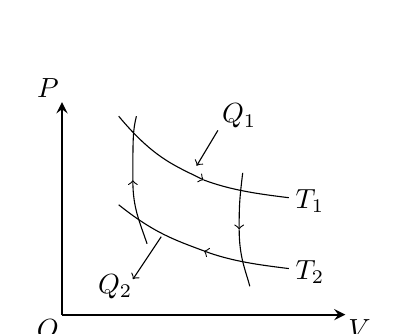
\begin{tikzpicture}[scale=0.9]
	\draw[thick, -stealth] (0,0)--(4,0);
	\draw[thick, -stealth] (0,0)--(0,3);
	\draw[->] (0.8,2.8) .. controls (1.3,2.2) and (1.6, 2.1) .. (2, 1.9);
	\draw (2,1.9) .. controls (2.4,1.75) and (2.8, 1.7) .. (3.2, 1.65);
	\draw (0.8,1.55) .. controls (1.3,1.15) and (1.6, 1.05) .. (2, 0.9);
	\draw[<-] (2,0.9) .. controls (2.4,0.75) and (2.8, 0.7) .. (3.2, 0.65);
	\draw[->] (1.2,1.0) .. controls (1.1, 1.3) and (1.0, 1.5) .. (1,1.9);
	\draw (1,1.9) .. controls (1, 2.5) and (1, 2.6) .. (1.05,2.8);
	\draw (2.65,0.4) .. controls (2.6, 0.6) and (2.5, 0.8) .. (2.5,1.2);
	\draw[<-] (2.5,1.2) .. controls (2.5, 1.5) and (2.5, 1.6) .. (2.55,2);
	\draw[<-] (1.9, 2.1)--(2.2,2.6);
	\draw[->] (1.4, 1.1)--(1.0,0.5);
	\node at (-0.2,-0.2) {$O$};
	\node at (-0.2,3.2) {$P$};
	\node at (4.2,-0.2) {$V$};
	\node at (3.5, 0.6) {$T_2$};
	\node at (3.5, 1.6) {$T_1$};
	\node at (2.5, 2.8) {$Q_1$};
	\node at (0.75,0.4) {$Q_2$};
\end{tikzpicture}
\label{fg:8}
\end{wrapfigure}

\hspace{-2cm}
\noindent 正卡诺循环:~\\对外做功$\Rightarrow \eta=\dfrac{W}{Q_1}=\dfrac{Q_1-Q_2}{Q_1}=1-\dfrac{T_2}{T_1}$;

~\\~\\~\\~\\

\begin{wrapfigure}{l}{.4\textwidth}
\vspace{-0.6cm}
\hspace{0.7cm}
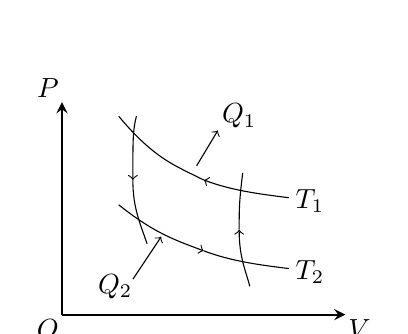
\begin{tikzpicture}[scale=0.9]
	\draw[thick, -stealth] (0,0)--(4,0);
	\draw[thick, -stealth] (0,0)--(0,3);
	\draw (0.8,2.8) .. controls (1.3,2.2) and (1.6, 2.1) .. (2, 1.9);
	\draw[<-] (2,1.9) .. controls (2.4,1.75) and (2.8, 1.7) .. (3.2, 1.65);
	\draw[->] (0.8,1.55) .. controls (1.3,1.15) and (1.6, 1.05) .. (2, 0.9);
	\draw (2,0.9) .. controls (2.4,0.75) and (2.8, 0.7) .. (3.2, 0.65);
	\draw (1.2,1.0) .. controls (1.1, 1.3) and (1.0, 1.5) .. (1,1.9);
	\draw[<-] (1,1.9) .. controls (1, 2.5) and (1, 2.6) .. (1.05,2.8);
	\draw[->] (2.65,0.4) .. controls (2.6, 0.6) and (2.5, 0.8) .. (2.5,1.2);
	\draw (2.5,1.2) .. controls (2.5, 1.5) and (2.5, 1.6) .. (2.55,2);
	\draw[->] (1.9, 2.1)--(2.2,2.6);
	\draw[<-] (1.4, 1.1)--(1.0,0.5);
	\node at (-0.2,-0.2) {$O$};
	\node at (-0.2,3.2) {$P$};
	\node at (4.2,-0.2) {$V$};
	\node at (3.5, 0.6) {$T_2$};
	\node at (3.5, 1.6) {$T_1$};
	\node at (2.5, 2.8) {$Q_1$};
	\node at (0.75,0.4) {$Q_2$};
\end{tikzpicture}
\label{fg:9}
\end{wrapfigure}

\hspace{-2cm}
\noindent 逆卡诺循环:

\noindent 制冷$\Rightarrow \eta=\dfrac{Q_2}{W}=\dfrac{Q_2}{Q_1-Q_2}=\dfrac{T_2}{T_1-T_2}$;

~\\~\\~\\~\\

\vspace{-0.5cm}
\noindent 8. 焓 Enthalpy: $H=E+pV$, $\mathrm{d}H=T\mathrm{d}S+V\mathrm{d}p$;
~\\\phantom{~~~}自由能 Helmholtz Free Energy: $F=E-TS$, $\mathrm{d}F=-S\mathrm{d}T-p\mathrm{d}V$;
~\\\phantom{~~~}吉布斯自由能 Gibbs Free Energy: $G=E-TS+pV$, $\mathrm{d}G=-S\mathrm{d}T+V\mathrm{d}p$.
~\\\phantom{~~~}配分函数: $Z=e^{-\beta F}$;
~\\\phantom{~~~}由$\mathrm{d}U\leqslant T\mathrm{d}S-p\mathrm{d}V$可知:等温等容:$\mathrm{d}F\leqslant 0$; 等温等压:$\mathrm{d}G\leqslant 0$.
~\\

\noindent 9. 黑体辐射: $P=\sigma T^4$;
~\\\phantom{~~~}维恩位移定律: $\lambda_{max}\cdot T=Constant$;
~\\\phantom{~~~}普朗克分布: $I(\nu, T)=\dfrac{2h\nu^3}{c^2}\dfrac{1}{e^{\frac{h\nu}{k_BT}-1}}$.
~\\
\begin{wrapfigure}{r}{.4\textwidth}
\vspace{-1.5cm}
\hspace{-0.5cm}
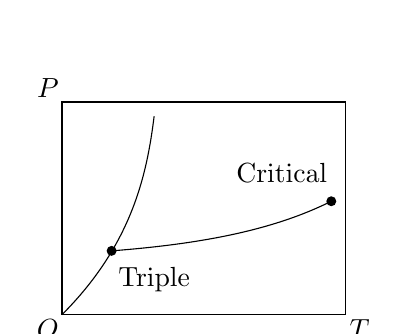
\begin{tikzpicture}[scale=0.9]
	\draw (0,0) rectangle (4,3);
	\draw (0,0) .. controls (1, 1) and (1.2, 2) .. (1.3, 2.8);
	\draw (0.7,0.9) .. controls (2,1.0) and (3,1.2) .. (3.8, 1.6);
	\fill (0.7,0.9) circle (2pt);
	\fill (3.8,1.6) circle (2pt);
	\node at (-0.2,-0.2) {$O$};
	\node at (-0.2, 3.2) {$P$};
	\node at (4.2,-0.2) {$T$};
	\node at (1.3,0.5) {Triple};
	\node at (3.1,2) {Critical};
\end{tikzpicture}
\label{fg:10}
\end{wrapfigure}

\vspace{-0.5cm}
\noindent 10. 相图:
~\\\phantom{~~~~} Critical临界点:气液之间无区别点;
~\\\phantom{~~~~} Triple三相电:气液固三相并存.
~\\

\noindent 11. 相变:$\mathrm{d}U=T\mathrm{d}S-p\mathrm{d}V$;
~\\\phantom{~~~~~}相变潜热:$L=T(S^{(2)}-S^{(1)})$; 体积突变:$\Delta V=V^{(2)}-V^{(1)}$.
~\\\phantom{~~~~~}一级相变:存在$L$和$\Delta V$; 二级相变(连续相变):无相变潜热和体积突变.
~\\

\addcontentsline{toc}{subsection}{4.3  Electronic Density of States}%add to contents
\noindent 12. 三维电子态密度
~\\\phantom{~~~~~}电子能量:$\varepsilon=\dfrac{p^2}{2m}=\dfrac{\hbar^2k^2}{2m}$, 每个量子态在$k$空间占据体积为$\dfrac{(2\pi)^3}{V}$,~\\\phantom{~~~~~}故态密度$N(E)=\dfrac{4\pi k^2\cdot\mathrm{d}k}{(2\pi)^3/V\cdot\mathrm{d}\varepsilon}$;
~\\\phantom{~~~~~}若考虑电子自旋$\times2$, 则$N(E)=\dfrac{2V}{(2\pi)^3}\dfrac{4\pi km}{\hbar^2}\propto\sqrt{E}$.

\newpage
\section{Optics}
\addcontentsline{toc}{subsection}{5.1  General Knowledge}%add to contents
\noindent1. 光速: $v=\dfrac{1}{\sqrt{\mu\varepsilon}}$.
~\\

\noindent2. 不确定度原理: $\Delta E\Delta\uptau\approx\hbar\Rightarrow\Delta\uptau\Delta\nu\approx 1$,
~\\\phantom{~~~~}相速度: $v_p=\dfrac{\omega}{k}$, 群速度: $v_g=\dfrac{\mathrm{d}\omega}{\mathrm{d}k}$,
~\\\phantom{~~~~}折射率: $n=\dfrac{c}{v}=\sqrt{\dfrac{\mu\varepsilon}{\mu_0\varepsilon_0}}\approx\sqrt{\dfrac{\varepsilon}{\varepsilon_0}}$.
~\\

\noindent3. 球面反射: $\dfrac{1}{s'}+\dfrac{1}{s}=\dfrac{1}{f}=\dfrac{2}{r}$, 放大率 magnification: $m=-\dfrac{s'}{s}$.
~\\\phantom{~~~~}球面折射: $\dfrac{n'}{s'}-\dfrac{n}{s}=\dfrac{n'-n}{r}$.
~\\\phantom{~~~~}薄透镜有: $\dfrac{1}{f'}=(n_0-1)(\dfrac{1}{r_1}-\dfrac{1}{r_2})$, ($n_0$为透镜折射率),
~\\\phantom{~~~~薄透镜有:~}$\dfrac{n'}{s'}-\dfrac{n}{s}=\dfrac{n_0-n}{r_1}+\dfrac{n'-n_0}{r_2}$,
~\\\phantom{~~~~薄透镜有:~}$\dfrac{1}{s'}-\dfrac{1}{s}=\dfrac{1}{f'}$.
~\\

\noindent4. 瑞利Rayleigh判据(中央最大与第一极小重叠)像可分辨:$\theta_R=1.22\dfrac{\lambda}{d}=0.61\dfrac{\lambda}{r}$,
~\\\phantom{~~~~}故艾里斑半径: $r=\theta_R f=(1.22\dfrac{\lambda}{D})f$.
~\\

\noindent5. 多普勒效应: $\dfrac{1}{\lambda_s}(v\pm v_s)=\dfrac{1}{\lambda_D}(v\pm v_D)$.
~\\

\addcontentsline{toc}{subsection}{5.2 Interference and Diffraction}%add to contents
\noindent6. 杨氏双缝干涉 (interference):
~\\\phantom{~~~~~~~~}最大: $d\sin\theta=m\lambda$, ($d$为双缝间距);
~\\\phantom{~~~~~~~~}最小: $d\sin\theta=(m+\dfrac{1}{2})\lambda$.
~\\\phantom{~~~~~~~~~~~~}$y_m=\dfrac{m\lambda L}{d}$, ($L$为缝屏间距).~\\

\noindent7. 单缝衍射 (diffraction):
~\\\phantom{~~~~~~~~}最大: $a\sin\theta=(m+\dfrac{1}{2})\lambda$, ($a$为缝宽).
~\\\phantom{~~~~~~~~}最小: $a\sin\theta=m\lambda$. 
~\\

\noindent8. 求成像最sharp时照相机的小孔半径: 
~\\\phantom{~~~~~~}即只有第一主极大在缝宽内 $y\approx a=D\cdot\theta$,
~\\\phantom{~~~~~~}而$a\cdot\sin\theta\approx a\cdot\theta=\lambda$, 故$a=\sqrt{\lambda D}$.
~\\

\noindent9. 光栅(gratting)衍射: 最大值$d\sin\theta=k\lambda$, 光栅常数$d=a+b$.~\\

\noindent10. 布拉格衍射: $2d\sin\theta=k\lambda$.~\\

\noindent11. 空气中薄膜(第一次反射有半波损失): $2nd=(m+\dfrac{1}{2})\lambda$.~\\

\noindent12.  迈克尔逊干涉仪:
~\\\phantom{~~~~~}插入折射率为$n$厚度为$L$的板:	$N=\dfrac{2L}{\lambda}$, $N'=\dfrac{2Ln}{\lambda}$,
~\\\phantom{~~~~~}故: $N'-N=\dfrac{2L}{\lambda}(n-1)$;
~\\\phantom{~~~~~}单纯移动镜面: $\Delta N=\dfrac{2L}{\lambda}$.
~\\

\noindent13. 牛顿环:

\begin{wrapfigure}{l}{.2\textwidth}
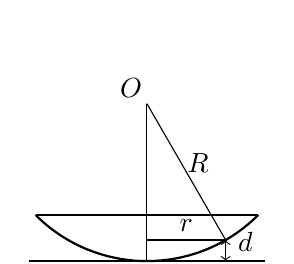
\begin{tikzpicture}[scale=1]
	\draw[thick] (-1.414,-1.414) arc (225:315:2);
	\draw[thick] (-1.414,-1.414) -- (1.414,-1.414);
	\draw (0,0)--(0,-2);
	\draw (0,0)--(1,-1.732);
	\draw (0,-1.732)--(1,-1.732);
	\draw [<->] (1,-1.732)--(1,-2);
	\draw [thick] (-1.5,-2)--(1.5,-2);
	\node at (-0.2,0.2) {$O$};
	\node at (0.65,-0.75) {$R$};
	\node at (0.5,-1.55) {$r$};
	\node at (1.25, -1.75) {$d$};
\end{tikzpicture}
\label{fg:11}
\end{wrapfigure}

\noindent$2d=(m+\dfrac{1}{2})\lambda$, $d=R-\sqrt{R^2-r^2}\approx\dfrac{r^2}{2R}$,
~\\故$r=\sqrt{R(m+\dfrac{1}{2})\lambda}$.

~\\~\\~\\

\noindent14. 通过偏振片: $I=\dfrac{I_0}{2}$;
~\\\phantom{~~~~~}马吕斯定律: $I=I_0\cos^2\theta$.
~\\

\begin{wrapfigure}{r}{.2\textwidth}
\vspace{-2cm}
\hspace{-2.5cm}
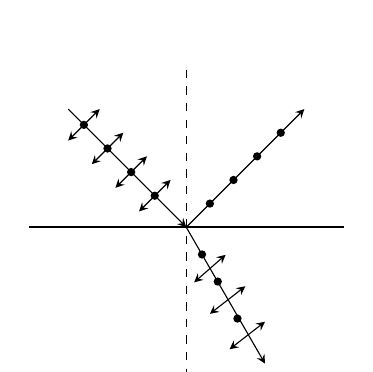
\begin{tikzpicture}[scale=1]
	\draw[thick] (-2,0)--(2,0);
	\draw[dashed] (0,2)--(0,-2);
	\draw[-stealth] (-1.5,1.5)--(0,0);
	\draw[-stealth] (0,0) -- (1.5,1.5);
	\draw[-stealth] (0,0) --(1,-1.732);
	\draw[stealth-stealth] (-1.5,1.1)--(-1.1,1.5);
	\fill (-1.3,1.3) circle (1.5pt);
	\draw[stealth-stealth] (-1.2,0.8)--(-0.8,1.2);
	\fill (-1.0,1.0) circle (1.5pt);
	\draw[stealth-stealth] (-0.9,0.5)--(-0.5,0.9);
	\fill (-0.7,0.7) circle (1.5pt);
	\draw[stealth-stealth] (-0.6,0.2)--(-0.2,0.6);
	\fill (-0.4,0.4) circle (1.5pt);
	\fill (0.3,0.3) circle (1.5pt);
	\fill (0.6,0.6) circle (1.5pt);
	\fill (0.9,0.9) circle (1.5pt);
	\fill (1.2,1.2) circle (1.5pt);
	\draw[stealth-stealth] (0.1,-0.7)--(0.5,-0.35);
	\fill (0.2,-0.346) circle (1.5pt);
	\fill (0.4,-0.69) circle (1.5pt);
	\draw[stealth-stealth] (0.3,-1.1)--(0.75,-0.75);
	\fill (0.65,-1.16) circle (1.5pt);
	\draw[stealth-stealth] (0.55,-1.55)--(1,-1.2);
\end{tikzpicture}
\label{fg:12}
\end{wrapfigure}

\noindent15. 斯涅耳定律: $n_1\sin\theta_1=n_2\sin\theta_2$;
~\\\phantom{~~~~~}布鲁斯特角: $\theta=\arctan\left(\dfrac{n_2}{n_1}\right)$,
~\\\phantom{~~~~~}布鲁斯特角时反射光和折射光的偏振方向如右图所示.
~\\

\noindent16. 干涉光强 $I=A_1^2+A_2^2+2A_1A_2\cos\delta$.
~\\

\noindent17. 光栅性能参数: <1> 角色散本领: $D_\theta=\dfrac{\delta\theta}{\delta\lambda}=\dfrac{K}{d\cos\theta}\Leftarrow(d\sin\theta=K\lambda\text{求导})$.
~\\\phantom{~~~~~光栅性能参数:~}<2> 线色散本领: $D_l=\dfrac{\delta l}{\delta\lambda}=D_\theta\cdot f=\dfrac{Kf}{d\cos\theta}$.
~\\\phantom{~~~~~光栅性能参数:~}<3> 色分辨本领: $R=\dfrac{\lambda}{\Delta\lambda}$,
~\\\phantom{~~~~~光栅性能参数:~<3>~}由$d\sin\theta=K(\lambda+\Delta\lambda)$和第一极小$d\sin\theta=(K+\dfrac{1}{N})\lambda$,
~\\\phantom{~~~~~光栅性能参数:~<3>~}得到$R=KN=\dfrac{Nd\sin\theta}{\lambda}$,
~\\\phantom{~~~~~光栅性能参数:~<3>~}其中$Nd$为光栅宽度,所以使用光栅时最好全照亮.
~\\\phantom{~~~~~光栅性能参数:~}<4> 色散范围(自由光谱范围):
~\\\phantom{~~~~~光栅性能参数:~<3>~}$K(\lambda+\Delta\lambda)=(K+1)\lambda\Rightarrow\Delta\lambda=\dfrac{\lambda}{K}=\dfrac{\lambda^2}{d\sin\theta}$.
~\\

\begin{wrapfigure}{r}{.2\textwidth}
\vspace{-0.8cm}
\hspace{-2.5cm}
\begin{tikzpicture}[scale=0.9]
	\draw[thick] (0,0) circle (2);
	\draw[thick] (0,0) ellipse (1.3 and 2);
	\draw[dashed] (0,2.5)--(0,-2.5);
	\draw[thick, -stealth] (0,0)--(0,2);
	\draw[thick, -stealth] (0,0)--(1.3,0);
	\fill (0,0) circle (1.5pt);
	\node at (0.25,1.7) {$v_o$};
	\node at (1.05,-0.25) {$v_e$};
	\node at (0.5,2.55) {光轴};
\end{tikzpicture}
\label{fg:13}
\end{wrapfigure}

\addcontentsline{toc}{subsection}{5.3 Crystal Optics}%add to contents
\noindent18. 晶体光学:
~\\\phantom{~~~~~}光轴: 不发生双折射.
~\\\phantom{~~~~~}主平面: 光线和光轴确定的平面.
~\\\phantom{~~~~~~~~~}$o$光垂直于主平面, $e$光平行于主平面.
~\\\phantom{~~~~~}正晶体: $v_o>v_e,~n_o<n_e$. (石英)
~\\\phantom{~~~~~}负晶体: $v_o<v_e,~n_o>n_e$. (方解石)
~\\\phantom{~~~~~}较快光的光矢量振动的方向$\rightarrow$快轴.
~\\\phantom{~~~~~}较慢光的光矢量振动的方向$\rightarrow$慢轴.
~\\

\noindent19. 正常色散柯西公式: $n=A+\dfrac{B}{\lambda^2}+\dfrac{C}{\lambda^4}$.
~\\\phantom{~~~~~}色散率: $\nu=\dfrac{\mathrm{d}n}{\mathrm{d}\lambda}=-\dfrac{2B}{\lambda^3}<0$;
~\\\phantom{~~~~~}而反常色散: $\nu>0$.
~\\

\noindent20. 散射强度: $I_\theta\propto\dfrac{1}{\lambda^4}$.
~\\\phantom{~~~~~}分子小: 瑞利散射(分子散射); 分子大: 米氏散射(延德尔散射).

\newpage
\section{Astrophysics and Relativity}
\addcontentsline{toc}{subsection}{6.1 Astrophysics}%add to contents
\noindent18. 晶体光学:
\noindent1. Parsec: 秒差距$=3.26$光年.
~\\\phantom{~~~~}$1^\circ=60'\text{~arcminute 角分}=3600''\text{~arcsecond 角秒}$.
~\\\phantom{~~~~}宇宙背景辐射: $\lambda T=C\Rightarrow T=\dfrac{C}{\lambda}\propto\dfrac{1}{r}$($\lambda\propto r$, $r$为宇宙半径)
~\\

\noindent2. 红移量: $z=\dfrac{\lambda_{ob}-\lambda_{em}}{\lambda_{em}}$, 当$v\ll c$时, 有$z\approx\dfrac{v}{c}=\beta$.
~\\

\noindent3. 哈勃定律: $v=H_0D\Rightarrow\dfrac{1}{H_0}$给出宇宙年龄.
~\\

\noindent4. 黑洞: Schwarzschid半径 $\dfrac{1}{2}mc^2-\dfrac{GMn}{r}=0\Rightarrow r=\dfrac{2GM}{c^2}$.
~\\

\addcontentsline{toc}{subsection}{6.2 Relativity}%add to contents
\noindent5. 洛伦兹变换: $\beta=\dfrac{v}{c}$, $\gamma=\dfrac{1}{\sqrt{1-\dfrac{v^2}{c^2}}}\approx1+\dfrac{1}{2}\dfrac{v^2}{c^2}\Rightarrow\dfrac{1}{\gamma}=1-\dfrac{1}{2}\dfrac{v^2}{c^2}$.
~\\\phantom{~~~~}四维坐标$(x_1,x_2,x_3,ict)$.
~\\\phantom{~~~~}坐标变换:
\[
	\left\{
		\begin{array}{l}
			x'=\dfrac{x-vt}{\sqrt{1-v^2 / c^2}},\\
			y'=y,~z'=z,\\
			t'=\dfrac{t-vx/c^2}{\sqrt{1-v^2/c^2}}.
		\end{array}
	\right.
\]
~\\\phantom{~~~~}速度变换:
\[
	\left\{
		\begin{array}{l}
			u_x=\dfrac{u'_x+v}{1+\dfrac{vu'_x}{c^2}},~u_y=\dfrac{u'_y\sqrt{1-\dfrac{v^2}{c^2}}}{1+\dfrac{vu'_x}{c^2}},~u_z=\dfrac{u'_z\sqrt{1-\dfrac{v^2}{c^2}}}{1+\dfrac{vu'_x}{c^2}};\\
			u'_x=\dfrac{u_x-v}{1-\dfrac{vu_x}{c^2}},~u'_y=\dfrac{u_y\sqrt{1-\dfrac{v^2}{c^2}}}{1-\dfrac{vu_x}{c^2}},~u'_z=\dfrac{u_z\sqrt{1-\dfrac{v^2}{c^2}}}{1+\dfrac{vu_x}{c^2}};\\
		\end{array}
	\right.
\]
~\\

\begin{wrapfigure}{r}{.2\textwidth}
\vspace{-1.2cm}
\hspace{-2,5cm}
\begin{tikzpicture}[scale=0.7]	
	\fill[color=gray!40] (-2.3,2.3)--(0,0)--(2.3,2.3);
	\fill[color=gray!40] (-2.3,-2.3)--(0,0)--(2.3,-2.3);
	\draw[thick, -stealth] (-3,0)--(3,0);
	\draw[thick, -stealth] (0,-3)--(0,3);
	\draw (-2.5,2.5)--(2.5,-2.5);
	\draw (-2.5,-2.5)--(2.5,2.5);
	\node[below right] at (3,0) {$r$};
	\node[above right] at (0,3) {$ct$};
	\node at (0,1.5) {绝对未来};
	\node at (0,-1.5) {绝对过去};	
	\node at (2,1) {类空};
\end{tikzpicture}
\label{fg:14}
\end{wrapfigure}

\noindent6. 间隔: $s^2=c^2\Delta t^2-(\Delta x)^2$.
~\\\phantom{~~~~~~~~}<1> $s^2=0$, 类光;
~\\\phantom{~~~~~~~~}<2> $s^2>0$, 类时, 可用低于光速的作用来连接;
~\\\phantom{~~~~~~~~}<3> $s^2<0$, 类空, 无因果关系,绝对异地;
~\\\phantom{~~~~}$E=mc^2=\dfrac{m_0c^2}{\sqrt{1-\dfrac{v^2}{c^2}}}=\dfrac{m_0c^2}{\sqrt{1-\dfrac{p^2c^2}{E^2}}}$
~\\\phantom{~~~~}$\Rightarrow E^2=p^2c^2+m_0^2c^4$.
~\\\phantom{~~~~}对于光子有$p=\dfrac{h}{\lambda}=\dfrac{h\nu}{c}=\dfrac{E}{c}$.
~\\

\noindent7. 相对论多普勒效应: $f'=\sqrt{\dfrac{1\pm\beta}{1\mp\beta}}f$(注意是$\beta$, 不是$\beta^2$)
~\\\phantom{~~~~}横向多普勒效应: $f'=\sqrt{1-\dfrac{v^2}{c^2}}f$(红移).
~\\

\noindent8. 电磁场:
\[
	\begin{array}{l}
		E'_x=E_x,~E'_y=\gamma(E_y-vB_z),~E'_z=\gamma(E_z+vB_y);\\
		B'_x=B_x,~B'_y=\gamma(B_y+\dfrac{v}{c^2}E_z),~B'_z=\gamma(B_z-\dfrac{v}{c^2}B_y).
	\end{array}
\]

\addcontentsline{toc}{subsection}{6.3 Cherenkov Radiation}%add to contents
\noindent9. 切连科夫辐射:
~\\\phantom{~~~~~~}当介质中光速小于带电粒子速度$v$时即$\dfrac{c}{n}<v$, 就会产生光子震波,如下图所示, 
~\\\phantom{~~~~~~}辐射角度满足$\cos\theta=\dfrac{c}{nv}=\dfrac{1}{n\beta}$, 其中$\beta=\dfrac{v}{c}$.

\begin{figure}[h]\fangsong
\centering
\begin{tikzpicture}[scale=0.7]	
	\draw[thick, -stealth] (0,0)--(7,0);
	\draw[red, thick, -stealth] (0.5,0)--(1.5,0);
	\draw[thick] (2,0)--(3,1.732)--(6,0)--(3,-1.732)--(2,0);
	\draw (2.93,1.53)--(3.1,1.45)--(3.18,1.6);
	\draw (2.93,-1.53)--(3.1,-1.45)--(3.18,-1.6);
	\draw[blue, thick] (2.3,0) arc (0:60:0.3);
	\node at (2.6, 0.4) {\color{blue}$\theta$};
	\draw[thick, -stealth, blue] (3,1.732)--(3.5,2.598);
	\draw[thick, -stealth, blue] (3.75,1.3)--(4.25,2.165);
	\draw[thick, -stealth, blue] (4.5,0.866)--(5,1.732);
	\draw[thick, -stealth, blue] (5.25,0.433)--(5.75,1.3);
	\draw[thick, -stealth, blue] (6,0)--(6.5,0.866);
	\draw[thick, -stealth, blue] (3,-1.732)--(3.5,-2.598);
	\draw[thick, -stealth, blue] (3.75,-1.3)--(4.25,-2.165);
	\draw[thick, -stealth, blue] (4.5,-0.866)--(5,-1.732);
	\draw[thick, -stealth, blue] (5.25,-0.433)--(5.75,-1.3);
	\draw[thick, -stealth, blue] (6,0)--(6.5,-0.866);
	\fill[red] (0.5,0) circle (3pt);	
	\node[above left] at (1.5,0) {\color{red}$v$};	
	\node at (2.1, 0.9) {$n$};
	\node at (7, 2) {\color{blue}光子震波};
\end{tikzpicture}
\label{fg:15}
\caption{切连科夫辐射}
\end{figure}

\newpage
\section{Quantum Mechanics}
\addcontentsline{toc}{subsection}{7.1 General Knowledge}%add to contents
\noindent1. 对易: $[AB,C]=A[B,C]+[A,C]B$; 标准差: $\sigma=\sqrt{\braket{j^2}-\braket{j}^2}$.
~\\\phantom{~~~~}泡利矩阵:
\[
	\sigma_x=
	\begin{pmatrix}
		0&1\\
		1&0\\
	\end{pmatrix},~
	\sigma_y=
	\begin{pmatrix}
		0&-i\\
		i&0\\
	\end{pmatrix},~
	\sigma_z=
	\begin{pmatrix}
		1&0\\
		0&-1\\
	\end{pmatrix}
\]
~\\\phantom{~~~~}$\vec{S}=\dfrac{\hbar}{2}\sigma$.
~\\

\noindent2. 含时薛定谔方程 $i\hbar\dfrac{\partial H}{\partial t}=\hat{H}\varPsi$, $\varPsi(t)=\varPsi(0)e^{-\frac{iHt}{\hbar}}$.
~\\\phantom{~~~~}定态薛定谔方程 $\hat{H}\varPsi=E\varPsi\Rightarrow-\dfrac{\hbar^2}{2m}\dfrac{\partial^2}{\partial x^2}\varPsi+V\varPsi=E\varPsi$.
~\\\phantom{~~~~}可观测量$Q$的期望值 $\braket{\hat{Q}}=\braket{\varPsi|\hat{Q}\varPsi}=\int\varPsi^*\hat{Q}\varPsi\mathrm{d}x$.
~\\

\noindent3. 动量对应算符 $p\rightarrow\dfrac{\hbar}{i}\dfrac{\partial}{\partial x}$或者$p\rightarrow-i\hbar\nabla$.
~\\\phantom{~~~~}$[\hat{x},\hat{p}]=i\hbar$.
~\\\phantom{~~~~}球谐函数$Y_l^m=\varTheta(\theta)e^{im\phi},~Y_0^0=\dfrac{1}{2}\sqrt{\dfrac{1}{\pi}}$.
~\\\phantom{~~~~}若波函数为$\cos m\phi=\dfrac{e^{im\phi}+e^{-im\phi}}{2}\Rightarrow$本征值为$m\hbar$和$-m\hbar$.
~\\

\noindent4. 标准边界条件:
\[
	\left\{
	\begin{array}{l}
		\varPsi(x)\text{连续};\\
		\dfrac{\mathrm{d}\varPsi}{\mathrm{d}x}\text{在势能不为无穷大处连续};
	\end{array}
	\right.
\]
~\\\phantom{~~~~}普朗克长度$l_p=\sqrt{\dfrac{\hbar G}{c^3}}\approx10^{-35}m$.
~\\\phantom{~~~~}概率流: $\vec{J}=\dfrac{\hbar}{2mi}(\varPsi^*\nabla\varPsi-\varPsi\nabla\varPsi^*)$.
~\\

\noindent5. 单态: $\ket{0~0}=\dfrac{1}{\sqrt{2}}\uparrow\downarrow-\dfrac{1}{\sqrt{2}}\downarrow\uparrow$.
~\\\phantom{~~~~}三重态:
\[
	\left\{
	\begin{array}{l}
		\ket{1~1}=\uparrow\uparrow\\
		\ket{1~0}=\dfrac{1}{\sqrt{2}}\uparrow\downarrow+\dfrac{1}{\sqrt{2}}\downarrow\uparrow\\
		\ket{1~{-1}}=\downarrow\downarrow
	\end{array}
	\right.
\]
~\\

\addcontentsline{toc}{subsection}{7.2 Stationary Schr\"odinger Equation}%add to contents
\noindent6. 无穷深势阱:
~\\\phantom{~~~~~~}在$0\leqslant x\leqslant a$, 波函数$\varPsi_n(x)=\sqrt{\dfrac{2}{a}}\sin(\dfrac{n\pi}{a}x),~n=1,2,3\dots$, 有$n-1$个节点, 
~\\\phantom{~~~~~~}能量$E_n=\dfrac{n^2\pi^2\hbar^2}{2ma^2}$.
~\\

\noindent7. 谐振子:
~\\\phantom{~~~~~~}能量$E_n=\hbar\omega(n+\dfrac{1}{2})$,
~\\\phantom{~~~~~~}波函数$\varPsi_0=\left(\dfrac{m\omega}{\pi\hbar}\right)^{\frac{1}{4}}e^{-\xi^2/2}$, $\xi=\sqrt{\dfrac{m\omega}{\hbar}}x$, $\varPsi_n$的奇偶性同$n$.
~\\

\noindent8. $\delta$函数势 $V=-\alpha\delta(x)$.
~\\\phantom{~~~~}考虑束缚态$E<0\Rightarrow x<0, -\dfrac{\hbar^2}{2m}\dfrac{\partial^2}{\partial x^2}\varPsi=E\varPsi$, 即$\dfrac{\partial^2}{\partial x^2}\varPsi=\kappa^2\varPsi,~\kappa=\dfrac{\sqrt{-2mE}}{\hbar}$,
~\\\phantom{~~~~}故$\varPsi(x)=Ae^{-\kappa x}+Be^{\kappa x}$. ($x\rightarrow-\infty$需收敛, 故$A=0$)
~\\\phantom{~~~~}同理$\varPsi(x)=Fe^{-\kappa x}~(x>0)$.
~\\\phantom{~~~~}边界条件$x=0$时有$B=F$,
~\\\phantom{~~~~}且$-\dfrac{\hbar^2}{2m}\displaystyle\int_{-\varepsilon}^{\varepsilon}\dfrac{\partial^2\varPsi}{\partial x^2}\mathrm{d}x+\int_{-\varepsilon}^{\varepsilon}V(x)\varPsi\mathrm{d}x=\int_{-\varepsilon}^{\varepsilon}E\varPsi(x)\mathrm{d}x$, (积分薛定谔方程)
~\\\phantom{~~~~~}$\Delta\left(\dfrac{\partial\varPsi}{\partial x}\right)=\dfrac{2m}{\hbar^2}\displaystyle\int_{-\varepsilon}^{\varepsilon}V(x)\varPsi(x)\mathrm{d}x=-\dfrac{2m\alpha}{\hbar^2}\varPsi(0)$.
~\\\phantom{~~~~}故$\Delta\left(\dfrac{\partial\varPsi}{\partial x}\right)=2B\kappa=-\dfrac{2m\alpha}{\hbar^2}B\Rightarrow\kappa=\dfrac{m\alpha}{\hbar^2}$,
~\\\phantom{~~~~}故$\varPsi(x)=\dfrac{\sqrt{m\alpha}}{\hbar}e^{-m\alpha |x|/\hbar^2},~E=-\dfrac{m\alpha^2}{2\hbar^2}$,
~\\\phantom{~~~~}可见只有一个束缚态解.

\begin{wrapfigure}{r}{.4\textwidth}
\vspace{-3cm}
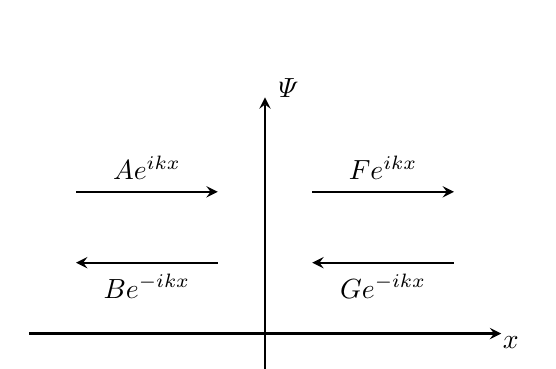
\begin{tikzpicture}[scale=0.6]	
	\draw[thick, -stealth] (-5,0)--(5,0);
	\draw[thick, -stealth] (0,-1)--(0,5);
	\draw[thick, -stealth] (-4,3)--(-1,3);
	\draw[thick, -stealth] (-1,1.5)--(-4,1.5);
	\draw[thick, -stealth] (1,3)--(4,3);
	\draw[thick, -stealth] (4,1.5)--(1,1.5);
	\node at (-2.5,3.5) {$Ae^{ikx}$};
	\node at (-2.5,1) {$Be^{-ikx}$};
	\node at (2.5,3.5) {$Fe^{ikx}$};
	\node at (2.5,1) {$Ge^{-ikx}$};
	\node at (5.2,-0.2) {$x$};
	\node at (0.5,5.2) {$\varPsi$};
\end{tikzpicture}
\label{fg:16}
\caption{边界反射与透射}
\end{wrapfigure}
~\\\phantom{~~~~}有限深势阱至少有1个束缚态解.
~\\\phantom{~~~~}共振透射$T=1\Rightarrow k'b=n\pi$.
~\\

\noindent9. 一阶微扰 $E_n^{(1)}=\bra{\varPsi_n^{(0)}}H'\ket{\varPsi_n^{(0)}}$.
~\\\phantom{~~~~}一阶波函数 $\varPsi_n^{(1)}=\displaystyle\sum_{m\not = n}\dfrac{\bra{\varPsi_m^{(0)}}H'\ket{\varPsi_m^{(0)}}}{E_n^0-E_m^0}\varPsi_m^0$.
~\\\phantom{~~~~}二阶微扰 $E_n^{(2)}=\displaystyle\sum_{m\not = n}\dfrac{|\bra{\varPsi_m^{(0)}}H'\ket{\varPsi_m^{(0)}}|^2}{E_n^0-E_m^0}=\bra{\varPsi_n^{(1)}}H'\ket{\varPsi_n^{(1)}}$.
~\\\phantom{~~~~}变分法: $\bra{\varPsi}H\ket{\varPsi}\leqslant E_g$, 
~\\\phantom{~~~~}试探函数一般可取$\varPsi(x)=Ae^{-bx^2}$或氢原子基态波函数$\varPsi_{100}=\dfrac{1}{\sqrt{\pi a^3}}e^{-r/a}$.
~\\

\noindent10. 不确定原理:
~\\\phantom{~~~~~~~~~~}$\sigma_A^2\sigma_B^2\leqslant(\dfrac{1}{2i}\braket{[A,B]})^2$.
~\\\phantom{~~~~~~~~~~}如$\sigma_x\sigma_p\leqslant\dfrac{\hbar}{2}$, $\sigma_E\sigma_t\leqslant\dfrac{\hbar}{2}$.
~\\\phantom{~~~~~~~~~~}气体密度$\rho\uparrow$, $\sigma_t\downarrow$, $\sigma_E\uparrow$, 故谱线越宽.
~\\

\addcontentsline{toc}{subsection}{7.3 Angular Momentum}%add to contents
\noindent11. 角动量: $L^2\varPsi=l(l+1)\hbar^2\varPsi$, $L_z\varPsi=m\hbar\varPsi$.
~\\\phantom{~~~~~}对易: $[r_i, r_j]=[p_i,r_j]=0,~[r_i, p_j]=i\hbar\delta_{ij}$,
~\\\phantom{~~~~~对易:~}$[L_x,L_y]=i\hbar L_z, [L^2, L_i]=0\Rightarrow[L^2,\vec{L}]=0$.
~\\\phantom{~~~~}令$L_\pm=L_x\pm iL_y,$ 则$[L_z,L_\pm]=\hbar L_\pm,~[L^2,L_\pm]=0$.
~\\\phantom{~~~~}且$L_\pm f_l^m=\hbar\sqrt{l(l+1)-m(m\pm1)}f_l^{m\pm 1}$.~\\

\noindent12. 氢原子: $E_n=-E_1(\dfrac{Z^2}{n^2}\dfrac{\mu}{\mu_e}),~E_1=\dfrac{q^4}{8\hbar^2\varepsilon_0^2}=12.6eV$.
~\\\phantom{~~~~~}一般情况$\mu\approx\mu_e\approx m_e$, 对于positronium, $\mu=\dfrac{m_e^2}{m_e+m_e}=\dfrac{1}{2}m_e$.
~\\\phantom{~~~~~}轨道电子速度$v_n=\dfrac{\alpha c}{n}$, 其中$\alpha$为精细结构常数$\dfrac{1}{137}$.
~\\\phantom{~~~~~}轨道半径$r_n\approx a_0(\dfrac{m_e}{\mu}\dfrac{n^2}{Z})$, 其中$a_0\approx 0.53\overset{\hspace{0.1cm}\circ}{A}$.
~\\\phantom{~~~~}基态波函数$\varPsi_{100}=\dfrac{1}{\sqrt{\pi a^3}}e^{-r/a}$, 第一激发态$\propto (1-\dfrac{r}{2a})e^{-r/2a}$.
~\\

\noindent13. 磁矩$\mu=-\dfrac{e}{2m}L$, 自旋$\mu_s=-\dfrac{ge}{2m}S$, 朗德因子$g=2$, 旋磁比$\gamma=\dfrac{\mu_s}{S}=-\dfrac{ge}{2m}$.
~\\

\addcontentsline{toc}{subsection}{7.4 Other Knowledge}%add to contents
\noindent14. Stern-Gerlach实验: Ag原子$5s^1$电子$\ket{\varPsi}=\dfrac{1}{\sqrt{2}}\uparrow\downarrow-\dfrac{1}{\sqrt{2}}\downarrow\uparrow$经过磁场分裂为两束.
~\\

\noindent15. 弗兰克-赫兹实验: 非弹性碰撞才会吸收电子能量.
~\\

\noindent16. 康普顿散射: $\Delta\lambda=\dfrac{h}{mc}(1-\cos\phi)$. (务必记住此公式)
~\\

\noindent17. 精细结构 split with $j$: <1> 相对论修正; <2> 自旋-轨道耦合.
~\\

\noindent18. 横截面微分 $D(\theta)=\dfrac{\mathrm{d}\sigma}{\mathrm{d}\Omega}$, 其中$\mathrm{d}\Omega=\sin\theta\mathrm{d}\theta\mathrm{d}\phi$.
~\\

\noindent19. 更多请参看量子力学笔记部分...

\newpage
\section{Solid State Physics}
\addcontentsline{toc}{subsection}{8.1 General Knowledge}%add to contents
\noindent1. $V=\vec{a}_1\cdot(\vec{a}_2\times\vec{a}_3)$. 
~\\\phantom{~~~~~}倒格子: $\vec{b}_1=2\pi\dfrac{\vec{a}_2\times\vec{a}_3}{\vec{a}_1\cdot(\vec{a}_2\times\vec{a}_3)},~\vec{b}_1=2\pi\dfrac{\vec{a}_3\times\vec{a}_1}{\vec{a}_1\cdot(\vec{a}_2\times\vec{a}_3)},~\vec{b}_1=2\pi\dfrac{\vec{a}_1\times\vec{a}_2}{\vec{a}_1\cdot(\vec{a}_2\times\vec{a}_3)}$.
~\\

\noindent2. 自由电子气: $E_F=\dfrac{\hbar^2k_F^2}{2m},~k_F=(3\rho\pi^2)^{\frac{1}{3}},~\rho$为电子数密度.
~\\\phantom{~~~~~自由~~}推导:在$T=0$时, 费米分布
$f_0(E)=\left\{\begin{array}{l}1, E\leqslant E_F\\0, E>E_F\end{array}\right.$,
~\\\phantom{~~~~自由电子气:~}态密度$N(E)=\dfrac{V}{2\pi^2}\left(\dfrac{2m}{\hbar^2}\right)^{\frac{3}{2}}E^{\frac{1}{2}}$
~\\\phantom{~~~~自由电子气:~态密度}$N=\displaystyle\int_0^\infty f_0(E)\cdot N(E)\mathrm{d}E=\dfrac{V}{2\pi^2}\left(\dfrac{2m}{\hbar^2}\right)^{\frac{3}{2}}\times\int_0^{E_F}E^{\frac{1}{2}}\mathrm{d}E$.
~\\\phantom{~~~~自由电子气:~}可得$E_F=\dfrac{\hbar^2}{2m}\left(\dfrac{3\pi^2 N}{V}\right)^{\frac{2}{3}}$, 故$k_F=\left(\dfrac{3\pi^2 N}{V}\right)^{\frac{1}{3}}$.
~\\

\noindent3. 有效质量: $\dfrac{\mathrm{d}^2E}{\mathrm{d}k^2}=\dfrac{\hbar^2}{m}$, 故$m^*=\dfrac{\hbar^2}{\left(\dfrac{\mathrm{d}^2E}{\mathrm{d}k^2}\right)}$.

\newpage

\section{Particle Physics}
\addcontentsline{toc}{subsection}{9.1 General Knowledge}%add to contents
\noindent1. $J/\varPsi$ meson 介子: 由一个charm quark和一个anti charm quark组成.
~\\\phantom{~~~~}Deutron: 氘核.
~\\\phantom{~~~~}自旋: 光子photon$=1$, 电子=$\dfrac{1}{2}$, 质子proton$=\dfrac{1}{2}$.
~\\

\noindent2. \[
	\text{hadron 强子}\left\{
	\begin{array}{l}
		\text{meson 介子(boson): a quark and an antiquark}.\\
		\text{baryon 重子 (fermion): 3 quarks}(\dfrac{1}{3}).
	\end{array}
	\right.
\]
\phantom{~~~~~~~~~~~~~~~~~~~~~~~~~~~~~~~~~~~~~~~~}baryon number $B(\pm1)$.
 \[
	\text{lepton 轻子}\left\{
	\begin{array}{l}
		\text{电子 electron} (e^-) \text{ 和电子中微子 electron neutrino} (\nu_e),\\
		\mu\text{子 muon} (\mu^-) \text{ 和}\mu\text{子中微子 muon neutrino} (\nu_\mu),\\
		\tau\text{子 tau} (\uptau) \text{ 和}\tau\text{子中微子 tau neutrino} (\nu_\tau).
	\end{array}
	\right.
\]
轻子数守恒: lepton number $L$ conservation.
~\\

\noindent3. 汤川秀树预言的介子是$\pi$介子, 不是$\mu$子.
~\\

\noindent4. $\mu$子衰变: $\mu^-\rightarrow e^-+\bar{\nu}_e+\nu_\mu$, $\mu^+\rightarrow e^++\nu_e+\bar{\nu}_\mu$.
~\\\phantom{~~~~}$\alpha$衰变: $^AN\rightarrow~^{A-4}L+~^4He$.
~\\\phantom{~~~~}$\beta$衰变: $\beta^-:~N\rightarrow O+e^-+\bar{\nu}_e~(n\rightarrow p+e^-+\bar{\nu}_e)$,
~\\\phantom{~~~~ib衰变:~}$\beta^+:~N\rightarrow O+e^++\nu_e~(p\rightarrow n+e^++\nu_e)$.
~\\\phantom{~~~~}$\beta^-$衰变更普遍,因为中子数量更多.

\newpage

\section{Atomic Physics and Nuclear Physics}
\addcontentsline{toc}{subsection}{10.1 Atomic Physics}%add to contents
\noindent1. $^{2S+1}L_J$, 锂 Lithium, 钠 Sodium.
~\\

\noindent2. 选择定则: $\Delta m_l=\pm 1, 0;~ \Delta l=\pm 1;~\Delta j=0,\pm1;~\Delta m_s=0$.
~\\\phantom{~~~~}洪特法则: <1> $S\uparrow,~E\downarrow$;
~\\\phantom{~~~~洪特法则:~}<2> $L\uparrow,~E\downarrow$;
~\\\phantom{~~~~洪特法则:~}<3> 如果壳层少于半满, $J=|L-S|,~E\downarrow$,
~\\\phantom{~~~~洪特法则:~<4>} 如果壳层多于半满, $J=L+S,~E\downarrow$,
~\\

\noindent3. 塞曼效应: $U=-\vec{\mu}\cdot\vec{B}=-\dfrac{ge}{2m}\vec{J}\cdot\vec{B}$.
~\\\phantom{~~~~}玻尔磁子: $\mu_B=\gamma\hbar=\dfrac{e\hbar}{2m}$.
~\\\phantom{~~~~}$h\nu'=h\nu+(m_2g_2-m_1g_1)\mu_B B$, 正常塞曼效应$S=0,~g_1=g_2=1,~\Delta m=0,\pm1$,
~\\\phantom{~~~~}故:$h\nu'=h\nu+
\begin{pmatrix}
	\mu_B B\\0\\-\mu_BB
\end{pmatrix}
\begin{array}{l}
	\sigma^+\text{左旋}\\\pi\text{线偏振}\\\sigma^-\text{右旋}
\end{array}
$
~\\\phantom{~~~~}$
\left\{
\begin{array}{l}
	\text{平行于}B\text{方向只能看到}\sigma^\pm~2\text{条}\\
	\text{垂直}B\text{方向可以看到}3\text{条}
\end{array}\right.
$
~\\

\noindent3. 斯塔克效应$(E)$: $U=\vec{p}\cdot\vec{E}=-qEr\cos\theta$.
~\\

\noindent4. X射线(exicite inner electrons of element near the nuclear)$\rightarrow$Auger transition俄歇跃迁.
~\\\phantom{~~~~}考虑shielding作用: $E=13.6eV(\dfrac{3}{4})(Z-1)^2$.
~\\

\noindent5. 激光(受激发射): 发射光子与入射光子有相同的$\omega$、$\phi$和偏振方向...

\begin{wrapfigure}{r}{.4\textwidth}
\hspace{-2cm}
\begin{tikzpicture}[scale=0.6]	
	\draw[thick] (0,0)--(4.5,0);
	\draw[thick] (2,3)--(4.5,3);
	\draw[thick] (0,5)--(4,5);
	\draw[thick,->] (1,0)--(1,5);
	\draw[thick,->] (3,5)--(3,3);
	\draw[thick,->] (3.5,3)--(3.5,0);
	\draw[thick,domain=3.7:4.8] plot(\x,{0.1*cos(20*\x r)+1.5});
	\draw[thick,->] (4.8,1.5)--(5.1,1.5);
	\node at (5.3, 0) {基态};
	\node at (5.65, 5.1) {short lived};
	\node at (7.05, 3.1) {metastable state};
	\node at (5.85, 1.6) {激光};
	\node at (-1.3, 3.1) {optical pump};
	\draw[thick,->] (-1,2.6)--(-1,-0.85);
	\node at (1, -1.35) {粒子数反转 (population inversion)};
\end{tikzpicture}
\label{fg:17}
\end{wrapfigure}
\vspace{-0.6cm}
~\\\phantom{~~~~}条件: 1. 相干coherent.
~\\\phantom{~~~~条件:~}2. 单色monochromatic.
~\\\phantom{~~~~条件:~}3. minimal divergence.
~\\\phantom{~~~~条件:~}4. high intensity.
~\\~\\~\\~\\\phantom{~~}6. 几种常用激光: 
~\\\phantom{~~~~~~~~}Diod Laser: active medium is semiconducting. (p-n结)
~\\\phantom{~~~~~~~~}Gas Laser: active medium is free gas. (电流$\stackrel{\text{激发}}{\longrightarrow}$atoms)
~\\

\addcontentsline{toc}{subsection}{10.2 Nuclear Physics}%add to contents
\noindent7. Nucleus is most likely to emit electrons in the direction opposite to the magnetic field.
~\\

\noindent8. $r\approx r_0A^{\frac{1}{3}}$, $r_0\approx 1.2 fm$, 结合能: $E_B=\displaystyle\sum_i m_i c^2-Mc^2$, 核子nucleon.
~\\

\noindent9. 半衰期: $N=N_0e^{-\lambda t},~R=-\dfrac{\mathrm{d}N}{\mathrm{d}t}=\lambda N$, $t_{1/2}=\dfrac{\ln 2}{\lambda}$,
~\\\phantom{~~~~}平均寿命mean life: $\uptau=\dfrac{1}{\lambda}$.
~\\\phantom{~~~~}若$\dfrac{\mathrm{d}N}{\mathrm{d}t}=-(\lambda_A+\lambda_B)N\Rightarrow N=N_0e^{-(\lambda_A+\lambda_B)N}$, 则$\dfrac{1}{t_{1/2}}=\dfrac{1}{t_{1/2}^A}+\dfrac{1}{t_{1/2}^B}$.
~\\

\noindent10. 单位$Gray=\dfrac{Energy}{Unit~mass}$, 即$1Gy=\dfrac{1J}{1kg}$.
~\\\phantom{~~~~}韧致辐射 Bremsstrahlung: 对电荷$P=\dfrac{q^2a^2}{6\pi\varepsilon_0c^3}\propto q^2\propto a^2$; 对电偶极子$P=\dfrac{\omega^4}{12\pi\varepsilon_0c^3}p^2$.
~\\

\noindent11. 卢瑟福散射: $\dfrac{1}{2}mv^2=k\dfrac{2e^2}{r}$.
~\\

\noindent12. $\dfrac{1}{\lambda}=R(\dfrac{1}{n^2}-\dfrac{1}{n'^2})$:
\vspace{0.2cm}
~\\\phantom{~~~~}$n=1$, 莱曼系;
~\\\phantom{~~~~}$n=2$, 巴耳末系$\left\{
	\begin{array}{l}
		H-\alpha\text{线},~3\rightarrow2\\
		H-\beta\text{线},~4\rightarrow2\\
		H-\gamma\text{线},~5\rightarrow2
	\end{array}
	\right.$
~\\\phantom{~~~~}$n=3$, 帕刑系.

\newpage
\section{Mathematics and Ohters}
\addcontentsline{toc}{subsection}{11.1 Mathematics Knowledge}%add to contents
\noindent1. $\displaystyle\sum n^2=\dfrac{n(n+1)(2n+1)}{6}$.
~\\

\noindent2. Fourier Series: $f(x)=\dfrac{a_0}{2}+\displaystyle\sum_{n=1}^\infty a_n\cos(\frac{n\pi x}{L})+b_n\sin(\frac{n\pi x}{L})$,
~\\\phantom{~~~~}其中$a_n=\dfrac{1}{L}\displaystyle\int_{-L}^L f(t)\cos(\dfrac{n\pi t}{L})\mathrm{d}t$, $b_n=\dfrac{1}{L}\displaystyle\int_{-L}^Lf(t)\sin(\dfrac{n\pi t}{L})\mathrm{d}t$.
~\\\phantom{~~~~}傅里叶变换: $f(\omega)=\dfrac{1}{\sqrt{2\pi}}\displaystyle\int_{-\infty}^\infty f(t)e^{-i\omega t}\mathrm{d}t$.~\\
\begin{wrapfigure}{r}{.4\textwidth}
\hspace{-1cm}
\vspace{-2cm}
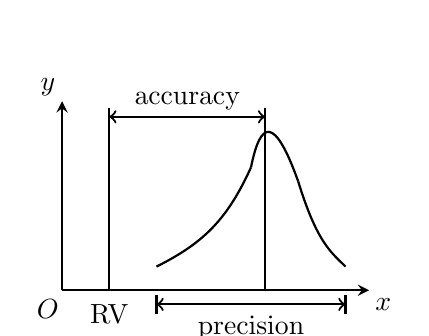
\begin{tikzpicture}[scale=0.6]	
	\draw[thick, -stealth] (1,0)--(7.5,0);
	\draw[thick, -stealth] (1,0)--(1,4);
	\draw[thick] (3,0.5) .. controls (4,1.0) and (4.5,1.5) .. (5,2.6);
	\draw[thick] (5,2.6) .. controls (5.2,3.6) and (5.5,3.7) .. (6,2.3);
	\draw[thick] (6,2.3) .. controls (6.4,1.0) and (6.7,0.8) .. (7,0.5);
	\draw[thick] (5.3,0.0)--(5.3,3.85);
	\draw[thick] (2,0.0) --(2,3.85);
	\draw[thick,<->] (2,3.67)--(5.3,3.67);
	\draw[thick,<->] (3,-0.3)--(7,-0.3);
	\draw[thick] (3,-0.1)--(3,-0.5);
	\draw[thick] (7,-0.1)--(7,-0.5);
	\node at (0.7,-0.4) {$O$};
	\node at (5,-0.8) {precision};
	\node at (2,-0.5) {RV};
	\node at (3.65, 4) {accuracy};
	\node at (7.8, -0.3) {$x$};
	\node at (0.7, 4.3) {$y$}; 
\end{tikzpicture}
\label{fg:18}
\end{wrapfigure}

\noindent3. 误差分析:
~\\\phantom{~~~~}
$
	\left.
	\begin{array}{l}
		\text{Accuracy}\\
		\text{Precision}
	\end{array}\right\}\text{区别}
$
~\\\phantom{~~~~}RV(Real Value)代表实际值.
~\\

\noindent4. 泊松分布: $P_\mu(\nu)=e^{-\mu}\dfrac{\mu^\nu}{\nu!}$,
~\\\phantom{~~~~}即$P(X=k)=e^{-\lambda}\dfrac{\lambda^k}{k!}$, 如下图所示.
~\\\phantom{~~~~}标准差$\sigma=\sqrt{\mu}$, 若重复$N$次, 则$\sigma_N=\dfrac{\sigma}{\sqrt{N}}$.
~\\\phantom{~~~~}$3-\sigma$原则对应概率: $0.6826$, $0.9544$, $0.9974$.

\begin{figure}[ht]
	\centering
	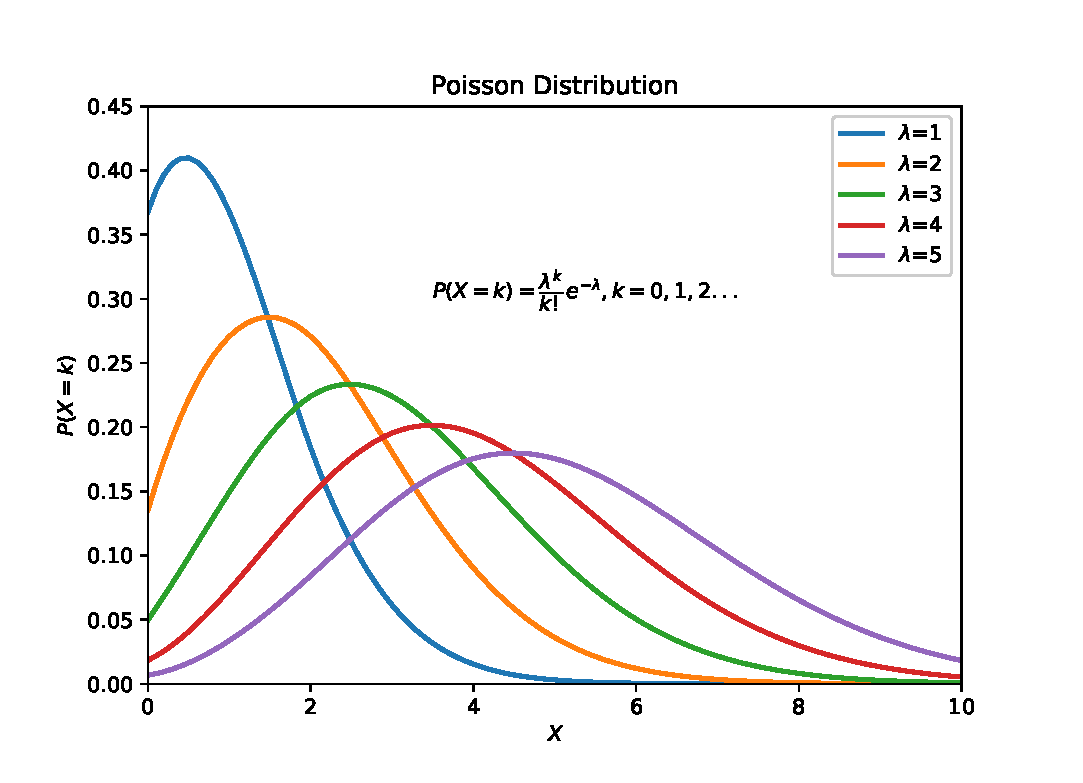
\includegraphics[width=.7\textwidth]{Poisson.eps}
	\label{fg:19}
	\caption{Poisson Distribution.}
\end{figure}

\addcontentsline{toc}{subsection}{11.2 Other Knowledge}%add to contents
\noindent5. 不确定度:
~\\\phantom{~~~~}<1> $x=a+b+\cdots \Rightarrow \mathrm{d}x=\mathrm{d}a+\mathrm{d}b+\cdots\Rightarrow(\delta x)^2=(\delta a)^2+(\delta b)^2+\cdots$;
~\\\phantom{~~~~}<2> $x=a\cdot b\cdots\Rightarrow\dfrac{\mathrm{d}x}{x}=\dfrac{\mathrm{d}a}{a}+\dfrac{\mathrm{d}b}{b}+\cdots\Rightarrow(\dfrac{\delta x}{x})^2=(\dfrac{\delta a}{a})^2+(\dfrac{\delta b}{b})^2+\cdots$.
~\\\phantom{~~~~}$N$次测量得到的值和不确定度分别为$x_i$和$\sigma_i$, 则每次的权重$\omega_i=\dfrac{1}{\sigma_i^2}$,
~\\\phantom{~~~~}则$x_{avg}=\dfrac{\sum\omega_ix_i}{\sum\omega_i},~\sigma_{avg}=\dfrac{1}{\sqrt{\sum\omega_i}}$.
~\\\phantom{~~~~}若多次测量均有$\omega_i=\omega$, 则$x_{avg}=\dfrac{\sum x_i}{N},~\sigma_{avg}=\dfrac{\sigma}{\sqrt{N}}$.
~\\

\noindent6. 原子核横截面积$\pi(10^{-14})^2m^2=10^{-28}m^2$;
~\\\phantom{~~~~}空气分子碰撞横截面积$\sigma=10^{-18}m^2$;
~\\\phantom{~~~~}空气粒子数密度$n=10^{25}m^{-3}$;
~\\\phantom{~~~~}空气分子平均自由程$l_p=\dfrac{1}{\sigma n}=10^{-7}m$.
\end{document}
